\section{Anwendung der Testgetriebenen Entwicklung}
\label{sec:awtdd}

In den nachfolgenden Abschnitten wird examplarisch an dem Objekt "`Job"', also der internen Repräsentation einer Stellenanzeige, die Testgetriebene Entwicklung mit praktischen Beispielen näher erläutert.
Besonderes Augenmerk soll dabei auf den Entwicklungsfluss von TDD gelegt werden. Zu dessen Verdeutlichung ist am Dokumentenrand die jeweilige Phase innerhalb des TDD-Zyklus zufinden (Red, Green, Refactor), dem die im Text gezeigten Codeabschnitte zuzuordnen sind.

Ziel dieses Kapitels wird es sein, einen Überblick über die Art und Weise zu erhalten, mit denen die verschiedenen Teilbereiche einer Webanwendung testgetrieben entwickelt werden können.
Die ersten drei Abschnitte richten sich an zwei der Grundbausteine einer MVC\foonnote{Model View Control} %TODO Link
Webanwendung, den Modell- und Controllertests. Im Dritten Abschnitt sehen wir, wie Test Doubles verwendet werden können, um Zugriffe auf externe Datenlieferanten zu simulieren. Danach betrachten wir die Anwendung aus Anwendersicht, und widmen wir uns der Implementierung von Akzeptanz- und Systemtests. % TODO Link
Zum Schluss gibt es einen Ausblick auf das Testen von Javascript-Ereignissen.

\section{Implementierung von Unit-Tests (Modelltests)}
\label{sec:awunit}

Ein Rails\index{Ruby-on-Rails}-Modell\index{Ruby-on-Rails!Modell}, wie in \ref{sec:railsconcepts} auf S. \pageref{sec:railsconcepts} beschrieben, repräsentiert die Daten der Anwendung und die Regeln, wie diese zu verändern sind. Bei Rails werden sie hauptsächlich dazu verwendet, um mit der zugrundeliegenden Datenbank\index{Datenbank}tabelle zu interagieren. Per Konvention von Rails findet hier die Hauptarbeit, also die Business-Logik, statt.

Fast jeder Unittest\index{Test!Unittest} bei Rails\index{Ruby-on-Rails} beinhaltet das Testen auf Validierung\index{Ruby-on-Rails!Validierung}skriterien seines korrespondierenden Modell\index{Ruby-on-Rails!Modell}s, d.h. wann eine Instanz dieses Modells gültig ist und damit gespeichert werden darf (man denke z.B. an Pflichtfelder für ein Modell "`Nutzer"` oder die Validierung des Formates seiner E-Mail-Adresse).

Diese Validierung\index{Ruby-on-Rails!Validierung}en werden durch das \glossar{ORM}-Framework ActiveRecord\index{ActiveRecord}, welches Rails\index{Ruby-on-Rails} standardmäßig nutzt, bereitgestellt.

\paragraph{1. Der Anfang}
\begin{figure}[htbp]
 \centering

 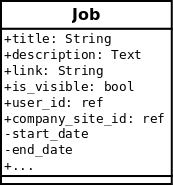
\includegraphics[width=0.3\textwidth]{./diagrams/job-erm.png}
 % job-erm.png: 173x186 pixel, 51dpi, 8.65x9.30 cm, bb=0 0 245 264
 \caption{Attribute des Modells "`Job"'}
  \label{fig:job-erm}
\end{figure}

Während der Analyse wurden die benötigten Attribute eines Jobs bestimmt. In Abbildung \ref{fig:job-erm} ist ein Fragment des Grobdesigns dargestellt, welches die Basisattribute der Jobs-Tabelle aufzeigt. Neben den einfachen Attributen, wie Title, Description und Link existieren auch Referenzen auf andere Objekte (d.h. dies stellen Fremdschlüssel zu anderen Tabellen dar), wie z.B. Schlagwörter (Tags), ein Besitzer einer Stellenanzeige (User) und so weiter.

Einer der häufigsten Wege, ein Modell\index{Ruby-on-Rails!Modell} und dessen Datenbank\index{Datenbank}schema zu generieren, ist die Nutzung des mitgelieferten Codegenerator\index{Code-Generator}s. Mittels des Kommandos:

\shadebox{
  rails generate model \textit{MODELLNAME} spalte1:datentyp1 spalte2:datentyp2 ...
}

generieren wir ein Modell\index{Ruby-on-Rails!Modell} mit dem angegebenen Modellnamen. Dazu geben wir paarweise die gewünschten Spaltennamen und deren Datentypen an (\texttt{string, text, datetime, references, integer, boolean, decimal}, ...).
\begin{lstlisting}
~/it-jobs$ rails generate model job title:string link:string \
    description:text user:references visible:boolean

      invoke  active_record
      create    db/migrate/20110828160636_create_jobs.rb
      create    app/models/job.rb
      invoke    test_unit
      create      test/unit/job_test.rb
      create      test/fixtures/jobs.yml

\end{lstlisting}
Mit der Anweisung uns ein Modell\index{Ruby-on-Rails!Modell} \texttt{job} mit den nachfolgenden Attributen zu generieren, hat Rails\index{Ruby-on-Rails} uns nun schon ein Stück Arbeit abgenommen. Dabei delegiert der Codegenerator\index{Code-Generator} \texttt{model} nun die Arbeit an den Codegenerator für ein ActiveRecord\index{ActiveRecord}-Model (erkennbar an dem \texttt{invoke active\_record}). Dieser wiederum generiert 2 Dateien und ruft seinerseits einen Codegenerator zum Generieren der Tests auf (\texttt{invoke test\_unit})

Es wurden erstellt:
\begin{itemize}
 \item Eine \textbf{Migration} (\verb|db/migrate/2011xxxxxx\_create\_jobs.rb|). Dies stellt eine datenbankunabhängige Repräsentation einer Änderung an der Struktur unserer Datenbank\index{Datenbank} dar. In diesem ist es die Erstellung einer Tabelle \texttt{jobs} (beachte: Plural!), mit den Spalten Titel, Link als String, Description als Textfeld, eine User\_ID als Referenz auf ein anderes Modell\index{Ruby-on-Rails!Modell} und die Sichtbarkeit der Stelle (visible),
 \item Die \textbf{Modelklasse} (\verb|app/models/job.rb|). Trotz unserer Definition der Spalten und deren Typen über die Kommandozeile, ist diese Klasse leer. Da wir ActiveRecord\index{ActiveRecord} verwenden, definieren wir die Attribute, die unser Modell\index{Ruby-on-Rails!Modell} hat, nicht in der Modellklasse, sondern ausschließ in der Datenbank\index{Datenbank}. Die Migration erspart uns die manuelle Arbeit, selbst in unserer Datenbank Spalten anzulegen. Bei Initialisierung eines Modells lädt ActiveRecord die Spalteninformationen aus der Datenbank und generiert dafür Getter- und Setter-Methoden (vgl. auch Abschnitt \ref{sec:railsconcepts}),
 \item die dazugehörige \textbf{Testklasse} (\verb|app/unit/job\_test.rb|) von Test/Unit (vgl. Abschnitt \ref{sec:rubyTestUnit})
 \item und \textbf{Fixtures}-Datei (\verb|test/fixtures/jobs.yml|), zur Definition von Testdaten\index{Test!Testdaten} (vgl. ebenfalls Abschnitt \ref{sec:rubyTestUnit}).
\end{itemize}

Die Migration liegt nun zwar vor, aber es existiert noch keine Datenbank\index{Datenbank} und demnach auch noch keine Tabelle mit dem Namen \texttt{jobs}.
Wir wollen Rails\index{Ruby-on-Rails} nun mitteilen, dass es die Migration anwenden soll, um damit die Datenbank\index{Datenbank} und Tabelle zu erstellen

Rails\index{Ruby-on-Rails} stellt uns mittels des Kommandozeilenwerkzeugs \textbf{\glossar{rake}} eine Schnittstelle zu unserer Anwendung bereit, mit der wir meist Wartungsaufgabe ausführen können. Rake\index{Ruby!Rake} erwartet die Angabe eines Tasks und optional die Angabe einer Umgebungsvariable für die Rails-Umgebung, in der der Test \index{Test}ausgeführt werden soll\footnote{Jede Umgebung verfügt normalerweise über eine eigene Datenbank\index{Datenbank}. standardmäßig befinden wir uns in der "`Development"'-Umgebung}.

\shadebox{  \centering
  rake \textit{TASK} [RAILS\_ENV=production]
}

Dazu weisen wir nun Rails\index{Ruby-on-Rails} an, alle offenen Migrationen auszuführen. Standardmäßig erstellt Rails dann selbstständig eine SQLite Datenbank\index{Datenbank} unter \texttt{db/development.sqlite3}.


\begin{lstlisting}[caption=Shell]
$ rake db:migrate

==  CreateJobs: migrating =========================
-- create_table(:jobs)
   -> 0.0020s
==  CreateJobs: migrated (0.0021s) ================
\end{lstlisting}

Danach können wir die Rails\index{Ruby-on-Rails}-Test-Suite\index{Test!Test-Suite} mithilfe eines weiteren Rake\index{Ruby!Rake}-Tasks auch schon ausführen. Dieser Rake-Task legt selbstständig eine Testdaten\index{Test!Testdaten}bank an, führt offene Migrationen darauf aus und führt dann alle vorhanden Tests aus.

\begin{lstlisting}[caption=Shell]
$ rake test
(in /home/zealot64/TEST)
Loaded suite /usr/lib/ruby/gems/1.8/gems/rake-0.8.7/lib/rake/rake_test_loader
Started
.
Finished in 0.043818 seconds.

1 tests, 1 assertions, 0 failures, 0 errors
\end{lstlisting}

Es wurde also schon ein Testfall\index{Test} erfolgreich ausgeführt, nämlich ein Dummytestfall von Rails\index{Ruby-on-Rails}:

\begin{ruby}[label={test/units/job\_test.rb}]
\PY{c+c1}{#test/unit/job\PYZus{}test.rb }
\PY{n+nb}{require} \PY{l+s+s1}{'test\PYZus{}helper'}

\PY{k}{class} \PY{n+nc}{JobTest} \PY{o}{<} \PY{n+no}{ActiveSupport}\PY{o}{::}\PY{n+no}{TestCase}
  \PY{c+c1}{# Replace this with your real tests.}
  \PY{n+nb}{test} \PY{l+s+s2}{"}\PY{l+s+s2}{the truth}\PY{l+s+s2}{"} \PY{k}{do}
    \PY{n}{assert} \PY{k+kp}{true}
  \PY{k}{end}
\PY{k}{end}
\end{ruby}
\label{list:bla}
\codecaption{Standardtest generiert durch Rails}


\paragraph{2. Testen auf Validierung}

Ein Feature von Rails\index{Ruby-on-Rails} umfassen die sogenannten Validierung\index{Ruby-on-Rails!Validierung}en. Diese stellen sicher, dass eine Instanz eines Modell\index{Ruby-on-Rails!Modell}s nur dann gespeichert wird, wenn es gewissen Kriterien entspricht. Viele der Validations sind vergleichbar mit den Datenbank\index{Datenbank}-Constraints einiger Datenbanken. Rails nutzt diese standardmäßig nicht, da es auch andere Persistenzsysteme unterstützt, wie z.B. Key-Value-Store oder sogenannte NoSQL Datenbanken. So stellt Rails die Konsistenz und referenzielle Integrität innerhalb der Applikationsschicht sicher.

Nun möchten wir sicherstellen, dass eine Stellenanzeige nur dann gespeichert wird, wenn sie einen Titel beinhaltet. Der Test \index{Test}dazu würde wie folgt lauten:

\begin{ruby}[label={test/units/job\_test.rb}]
\PY{n+nb}{require} \PY{l+s+s1}{'test\PYZus{}helper'}

\PY{k}{class} \PY{n+nc}{JobTest} \PY{o}{<} \PY{n+no}{ActiveSupport}\PY{o}{::}\PY{n+no}{TestCase}
  \PY{n+nb}{test} \PY{l+s+s2}{"}\PY{l+s+s2}{ein Job muss einen Titel haben}\PY{l+s+s2}{"} \PY{k}{do}
    \PY{n}{job} \PY{o}{=} \PY{n+no}{Job}\PY{o}{.}\PY{n}{new}
    \PY{n}{job}\PY{o}{.}\PY{n}{title} \PY{o}{=} \PY{k+kp}{nil}
    \PY{n}{assert} \PY{o}{!}\PY{n}{job}\PY{o}{.}\PY{n}{save}
  \PY{k}{end}
\PY{k}{end}
\end{ruby}
\codecaption{Test auf Vorhandensein eines Titels}
\tddred
Zuerst instanziieren wir einen Job und geben ihm explizit einen leeren Titel, um das Testziel nochmal herauszustellen. Danach rufen wir die \texttt{save}-Methode auf, die prüft, ob alle Validierung\index{Ruby-on-Rails!Validierung}skriterien erfolgt sind und speichert das Objekt persistent in der Datenbank\index{Datenbank} im Erfolgsfall. Dann gibt \texttt{save} ein \texttt{true} zurück, andernfalls, d.h. wenn die Validierung fehlschlug, \texttt{false}.
Der Ablauf ist in der Abbildung \ref{fig:activerecordsave} noch einmal erläutert.

\begin{figure}[hbp]
 \centering
 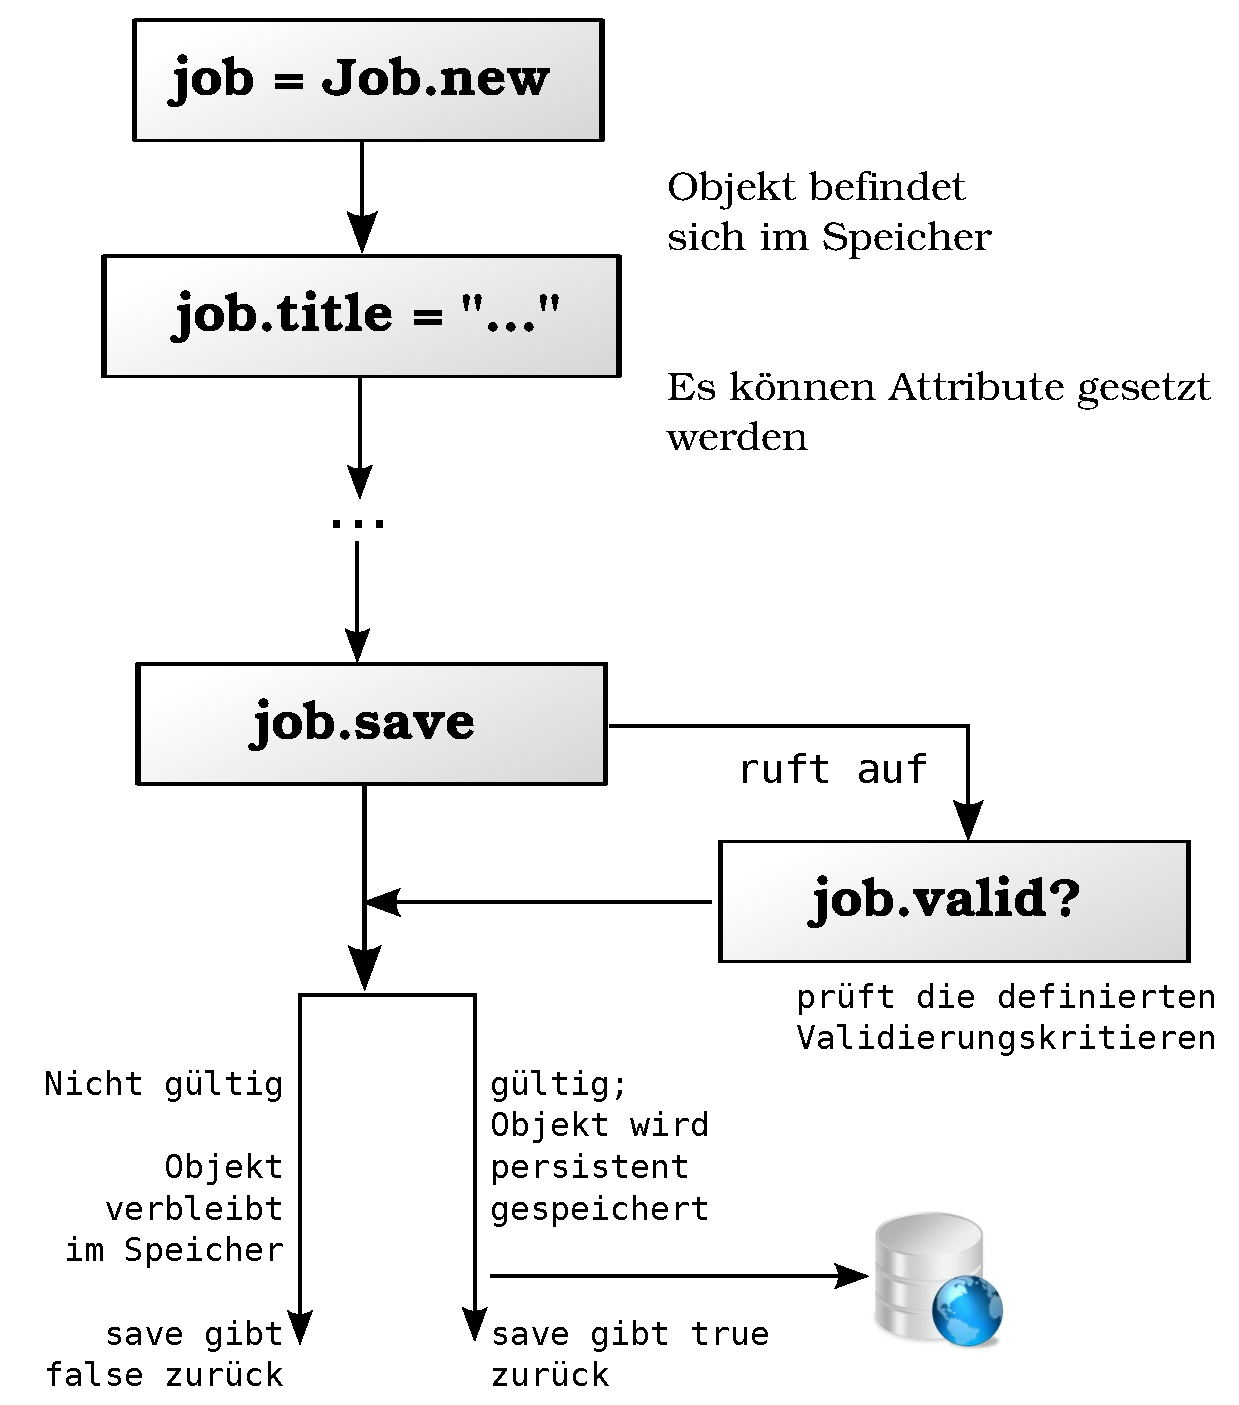
\includegraphics[width=0.65\textwidth]{./diagrams/activerecord-save.pdf}
 % activerecord-save.pdf: 595x675 pixel, 72dpi, 20.99x23.81 cm, bb=0 0 595 675
 \caption{Funktionsweise von save bei ActiveRecord Objekten}
 \label{fig:activerecordsave}
\end{figure}

Da wir noch keine Validierung\index{Ruby-on-Rails!Validierung}skriterien implementiert haben, gibt \texttt{save} \texttt{true} zurück und die Zusicherung schlägt fehl.

Unser nächstes Ziel ist es nun, mit so wenig Code wie möglich den Test \index{Test}bestehen zu lassen. Das können wir mittels der eingebauten wie schon erwähnten Validierung\index{Ruby-on-Rails!Validierung}en:

\begin{ruby}[label=app/models/job.rb]
\PY{k}{class} \PY{n+nc}{Job} \PY{o}{<} \PY{n+no}{ActiveRecord}\PY{o}{::}\PY{n+no}{Base}
  \PY{n}{validates} \PY{l+s+ss}{:title}\PY{p}{,} \PY{l+s+ss}{:presence} \PY{o}{=}\PY{o}{>} \PY{k+kp}{true}
\PY{k}{end}
\end{ruby}
\codecaption{Implementierung der Validierung in die Klasse Job}
\texttt{validates} ist eine Funktion aus der ActiveRecord\index{ActiveRecord} Bibliothek, die zwei Parameter entgegennimmt: Der erste ist die Spalte, auf der sich die Validierung\index{Ruby-on-Rails!Validierung} bezieht, als Zweites folgt eine Liste an Validierungskriterien. Hier ist das Kriterium \texttt{presence}, also das Vorhandensein eines nicht-leeren Wertes für diese Spalte. Weitere Kriterien sind z.B. Format, Länge, Minimum, Maximum oder auch selbst definierte Kriterien.

\tddgreen
Nach erneuter Ausführung der Testsuite besteht der Test \index{Test}nun. Jetzt folgt die Refaktorisierung\index{Refaktorisierung}sphase. Der Programmcode lässt sich nicht weiter vereinfachen. Aber der Testcode ist ausdrücklich nicht von Refaktorisierungen befreit und eine Refaktorisierung wäre z.B.:
\tddrefactor
\begin{ruby}[label=test/unit/job\_test.rb]
\PY{n+nb}{test} \PY{l+s+s2}{"}\PY{l+s+s2}{ein Job muss einen Titel haben}\PY{l+s+s2}{"} \PY{k}{do}
  \PY{n}{job} \PY{o}{=} \PY{n+no}{Job}\PY{o}{.}\PY{n}{new} \PY{l+s+ss}{:title} \PY{o}{=}\PY{o}{>} \PY{k+kp}{nil}
  \PY{n}{assert} \PY{o}{!}\PY{n}{job}\PY{o}{.}\PY{n}{save}
\PY{k}{end}
\end{ruby}
\codecaption{refaktorisierter Test}

Nun wollen wir dasselbe für das Feld E-Mail tun, hierbei aber nicht nur das Vorhandensein prüfen, sondern auch das Format.

\begin{ruby}[label=test/unit/job\_test.rb]
\PY{n+nb}{test} \PY{l+s+s2}{"}\PY{l+s+s2}{ein Job muss eine gültige E-Mail haben}\PY{l+s+s2}{"} \PY{k}{do}
  \PY{n}{job} \PY{o}{=} \PY{n+no}{Job}\PY{o}{.}\PY{n}{new} \PY{l+s+ss}{:email} \PY{o}{=}\PY{o}{>} \PY{l+s+s2}{"}\PY{l+s+s2}{invalid\PYZus{}email}\PY{l+s+s2}{"}
  \PY{n}{assert} \PY{o}{!}\PY{n}{job}\PY{o}{.}\PY{n}{save}
\PY{k}{end}
\end{ruby}
\tddred
Die Implementierung wäre dann:
\begin{ruby}[label=app/models/job.rb]
\PY{k}{class} \PY{n+nc}{Job} \PY{o}{<} \PY{n+no}{ActiveRecord}\PY{o}{::}\PY{n+no}{Base}
  \PY{n}{validates} \PY{l+s+ss}{:email}\PY{p}{,} \PY{l+s+ss}{:format} \PY{o}{=}\PY{o}{>} \PY{l+s+sr}{/}\PY{l+s+sr}{\PYZca{}[}\PY{l+s+sr}{\PYZbs{}}\PY{l+s+sr}{w}\PY{l+s+sr}{\PYZbs{}}\PY{l+s+sr}{d\PYZus{}}\PY{l+s+sr}{\PYZbs{}}\PY{l+s+sr}{-]+@[}\PY{l+s+sr}{\PYZbs{}}\PY{l+s+sr}{w}\PY{l+s+sr}{\PYZbs{}}\PY{l+s+sr}{d\PYZus{}}\PY{l+s+sr}{\PYZbs{}}\PY{l+s+sr}{-]}\PY{l+s+sr}{\PYZbs{}}\PY{l+s+sr}{.[}\PY{l+s+sr}{\PYZbs{}}\PY{l+s+sr}{w}\PY{l+s+sr}{\PYZbs{}}\PY{l+s+sr}{d]\PYZob{}2,3\PYZcb{}\$}\PY{l+s+sr}{/}
  \PY{o}{.}\PY{n}{.}\PY{o}{.}
\PY{k}{end}
\end{ruby}
\tddgreen
Eine Refaktorisierung\index{Refaktorisierung} ist aufgrund der Einfachheit des Beispiels hier nur gering möglich. Man könnte z.B. den regulären Ausdruck, der das Format der E-Mail Adresse beschreibt in eine neue Klasse oder zumindest eine Konstante auslagern. Wir wählen eine Konstante, die beim Laden von Rails\index{Ruby-on-Rails} bereitgestellt wird.
\tddrefactor
\begin{ruby}[label=config/initializers/regex.rb und app/models/job.rb]
\PY{c+c1}{# config/initializers/regex.rb}
\PY{n+no}{REGEX\PYZus{}EMAIL\PYZus{}FORMAT} \PY{o}{=} \PY{l+s+sr}{/}\PY{l+s+sr}{\PYZca{}[}\PY{l+s+sr}{\PYZbs{}}\PY{l+s+sr}{w}\PY{l+s+sr}{\PYZbs{}}\PY{l+s+sr}{d\PYZus{}}\PY{l+s+sr}{\PYZbs{}}\PY{l+s+sr}{-]+@[}\PY{l+s+sr}{\PYZbs{}}\PY{l+s+sr}{w}\PY{l+s+sr}{\PYZbs{}}\PY{l+s+sr}{d\PYZus{}}\PY{l+s+sr}{\PYZbs{}}\PY{l+s+sr}{-]}\PY{l+s+sr}{\PYZbs{}}\PY{l+s+sr}{.[}\PY{l+s+sr}{\PYZbs{}}\PY{l+s+sr}{w}\PY{l+s+sr}{\PYZbs{}}\PY{l+s+sr}{d]\PYZob{}2,3\PYZcb{}\$}\PY{l+s+sr}{/}

\PY{c+c1}{# app/models/job.rb}
\PY{k}{class} \PY{n+nc}{Job} \PY{o}{<} \PY{n+no}{ActiveRecord}\PY{o}{::}\PY{n+no}{Base}
  \PY{n}{validates} \PY{l+s+ss}{:email}\PY{p}{,} \PY{l+s+ss}{:format} \PY{o}{=}\PY{o}{>} \PY{n+no}{REGEX\PYZus{}EMAIL\PYZus{}FORMAT}
    \PY{o}{.}\PY{n}{.}\PY{o}{.}
\PY{k}{end}
\end{ruby}
\codecaption{Auslagerung des Regulären Ausdrucks in einen Initalisierer}
Ein erneutes Ausführen der Tests betätigt den Erfolg der Refaktorisierung\index{Refaktorisierung}.

\paragraph{3. Refaktorisierungen der Testklasse}
Nun fehlt aber noch die Definition eines Positiv-Beispiel für einen gültigen Job.

\begin{ruby}[label=test/unit/job\_test.rb]
...
\PY{n+nb}{test} \PY{l+s+s2}{"}\PY{l+s+s2}{ein vollstaendiger Job muss gueltig sein}\PY{l+s+s2}{"} \PY{k}{do}
  \PY{n}{job} \PY{o}{=} \PY{n+no}{Job}\PY{o}{.}\PY{n}{new} \PY{l+s+ss}{:title} \PY{o}{=}\PY{o}{>} \PY{l+s+s2}{"}\PY{l+s+s2}{Rails Entwickler}\PY{l+s+s2}{"}\PY{p}{,} \PY{l+s+ss}{:email} \PY{o}{=}\PY{o}{>} \PY{l+s+s2}{"}\PY{l+s+s2}{stefan@mail.com}\PY{l+s+s2}{"}
  \PY{n}{assert\PYZus{}valid} \PY{n}{job}
\PY{k}{end}
\end{ruby}
\tddgreen
Dieser Test \index{Test}besteht sofort, macht also genau genommen keine weitere Aussage über unser System. Nach der "`reinen"' Testgetriebene\index{TDD}n Lehre sollte dieser entfernt werden. Es ist allerdings eine gute Strategie, bei Validierung\index{Ruby-on-Rails!Validierung}en mindestens ein Beispiel zu präsentieren, das den Kriterien entspricht und angenommen wird. Nichtsdestotrotz können wir nun refaktorisieren. Insbesondere unsere Testfunktionen enthalten unnötige Redundanzen:

\begin{ruby}[label=test/unit/job\_test.rb]
\PY{n+nb}{test} \PY{l+s+s2}{"}\PY{l+s+s2}{ein Job muss einen Titel haben}\PY{l+s+s2}{"} \PY{k}{do}
  \PY{n}{job} \PY{o}{=} \PY{n+no}{Job}\PY{o}{.}\PY{n}{new} \PY{l+s+ss}{:title} \PY{o}{=}\PY{o}{>} \PY{k+kp}{nil}
  \PY{n}{assert} \PY{o}{!}\PY{n}{job}\PY{o}{.}\PY{n}{save}
\PY{k}{end}
\PY{n+nb}{test} \PY{l+s+s2}{"}\PY{l+s+s2}{ein Job muss eine gültige E-Mail haben}\PY{l+s+s2}{"} \PY{k}{do}
  \PY{n}{job} \PY{o}{=} \PY{n+no}{Job}\PY{o}{.}\PY{n}{new} \PY{l+s+ss}{:email} \PY{o}{=}\PY{o}{>} \PY{l+s+s2}{"}\PY{l+s+s2}{invalid\PYZus{}email}\PY{l+s+s2}{"}
  \PY{n}{assert} \PY{o}{!}\PY{n}{job}\PY{o}{.}\PY{n}{save}
\PY{k}{end}
\PY{n+nb}{test} \PY{l+s+s2}{"}\PY{l+s+s2}{ein vollstaendiger Job muss gueltig seinn}\PY{l+s+s2}{"} \PY{k}{do}
  \PY{n}{job} \PY{o}{=} \PY{n+no}{Job}\PY{o}{.}\PY{n}{new} \PY{l+s+ss}{:title} \PY{o}{=}\PY{o}{>} \PY{l+s+s2}{"}\PY{l+s+s2}{Rails Entwickler}\PY{l+s+s2}{"}\PY{p}{,} \PY{l+s+ss}{:email} \PY{o}{=}\PY{o}{>} \PY{l+s+s2}{"}\PY{l+s+s2}{stefan@mail.com}\PY{l+s+s2}{"}
  \PY{n}{assert\PYZus{}valid} \PY{n}{job}
\PY{k}{end}
\end{ruby}
\codecaption{Alle bisherigen Testmethoden in der Klasse JobTest}
\tddrefactor
In allen drei Methoden wird ein Job instanziiert und lediglich verschiedene Attribute überprüft. Auch haben unsere ersten beiden Tests keine gültige Aussage mehr, da der jeweilige Job sowieso nicht gültig ist, da jeweils das andere Attribut fehlt\footnote{Im ersten Test ist nicht nur der Titel nicht gesetzt, sondern auch die E-Mail entspricht nicht dem Format}. Es ist also höchste Zeit, die Tests zu refaktorisieren. Dies geschieht am besten durch die Verwendung einer Testdaten\index{Test!Testdaten}-Generation, z.B. den eingebauten Fixtures, die Rails\index{Ruby-on-Rails} uns bei der Codegeneration schon mit generiert hatte. Dabei definieren wir zentralisiert unsere (gültigen) Testdaten, die von Rails vor jedem einzelnen Test in der Datenbank\index{Datenbank} bereitgestellt werden (Mehr zu Fixtures in Abschnitt \ref{sec:rubyTestUnit}):

\begin{ruby}[label=test/fixtures/jobs.yml]
\PY{l+lScalar+lScalarPlain}{valid\PYZus{}job}\PY{p+pIndicator}{:}
  \PY{l+lScalar+lScalarPlain}{title}\PY{p+pIndicator}{:} \PY{l+lScalar+lScalarPlain}{Rails}\PY{l+lScalar+lScalarPlain}{ }\PY{l+lScalar+lScalarPlain}{Entwickler}
  \PY{l+lScalar+lScalarPlain}{email}\PY{p+pIndicator}{:} \PY{l+lScalar+lScalarPlain}{stefan@mail.com}
  \PY{l+lScalar+lScalarPlain}{link}\PY{p+pIndicator}{:} \PY{l+s}{"}\PY{l+s}{http://www.example.com/jobs}\PY{l+s}{"}
  \PY{l+lScalar+lScalarPlain}{visible}\PY{p+pIndicator}{:} \PY{l+lScalar+lScalarPlain}{true}
  \PY{l+lScalar+lScalarPlain}{...}
\PY{l+lScalar+lScalarPlain}{invisible\PYZus{}job}\PY{p+pIndicator}{:}
  \PY{l+lScalar+lScalarPlain}{title}\PY{p+pIndicator}{:} \PY{l+lScalar+lScalarPlain}{Rails}\PY{l+lScalar+lScalarPlain}{ }\PY{l+lScalar+lScalarPlain}{Entwickler}
  \PY{l+lScalar+lScalarPlain}{visible}\PY{p+pIndicator}{:} \PY{l+lScalar+lScalarPlain}{false}
  \PY{l+lScalar+lScalarPlain}{...}
\end{ruby}
\codecaption{Fixtures Testdaten für zwei Jobs}

Nun können wir diese Fixtures in unseren Tests verwenden und das ganze in einer \texttt{setup}-Methode, die vor jedem Testfall\index{Test} aufgerufen wird, laden:
\tddrefactor
\begin{ruby}[label=test/unit/job\_test.rb]
\PY{k}{class} \PY{n+nc}{JobTest} \PY{o}{<} \PY{n+no}{ActiveSupport}\PY{o}{::}\PY{n+no}{TestCase}
  \PY{n}{setup} \PY{k}{do}
    \PY{n+nv+vi}{@job} \PY{o}{=} \PY{n}{jobs} \PY{l+s+ss}{:valid\PYZus{}job}
    \PY{c+c1}{# Dies lädt den Job mit dem Schlüssel "valid\PYZus{}job" und schreibt ihn }
    \PY{c+c1}{#  in die Instanzvariable @job der Testklasse}
  \PY{k}{end}
  \PY{n+nb}{test} \PY{l+s+s2}{"}\PY{l+s+s2}{stelle sicher, dass die Fixtures valide sind}\PY{l+s+s2}{"} \PY{k}{do}
    \PY{n}{assert\PYZus{}valid} \PY{n+nv+vi}{@job}
  \PY{k}{end}
  \PY{n+nb}{test} \PY{l+s+s2}{"}\PY{l+s+s2}{ein Job muss einen Titel haben}\PY{l+s+s2}{"} \PY{k}{do}
    \PY{n+nv+vi}{@job}\PY{o}{.}\PY{n}{title} \PY{o}{=} \PY{k+kp}{nil}
    \PY{n}{assert} \PY{o}{!}\PY{n+nv+vi}{@job}\PY{o}{.}\PY{n}{save}
  \PY{k}{end}
  \PY{n+nb}{test} \PY{l+s+s2}{"}\PY{l+s+s2}{ein Job muss eine gültige E-Mail haben}\PY{l+s+s2}{"} \PY{k}{do}
    \PY{n+nv+vi}{@job}\PY{o}{.}\PY{n}{email} \PY{o}{=} \PY{l+s+s2}{"}\PY{l+s+s2}{invalid\PYZus{}email}\PY{l+s+s2}{"}
    \PY{n}{assert} \PY{o}{!}\PY{n+nv+vi}{@job}\PY{o}{.}\PY{n}{save}
  \PY{k}{end}
\PY{k}{end}
\end{ruby}
\codecaption{Finale Job-Test Klasse nach Refaktorisierung}



Am Ende dieser Refaktorisierung\index{Refaktorisierung}en ist es notwendig, die Tests noch einmal auszuführen.
\tddgreen
Danach würde die Implementierung einer nächsten Teilanforderung sein.

In diesem Abschnitt war zu sehen, dass die Testgetriebene\index{TDD} Entwicklung das Arbeiten und Testen in kleinen Schritten favorisiert.

\subsection{Implementierung von Controller-Tests (functional tests)}

Neben den Unittests stellt Ruby on Rails eine weitere Testart nativ bereit. Technisch gesehen handelt es sich bei diesen Functional Tests aber auch um Unittests, da deren Testobjekt ein Controller ist. 
Ein Controller hat bei Ruby on Rails die Aufgabe, Anfragen für bestimmte Routen, also Web-Adressen, anzunehmen, die Arbeit an eine Modelklasse auszulagern, und eine View aufzurufen, die letztendlich HTML-Code generiert.

Im ersten Beispiel wollen wir testen, dass ein Gast-Nutzer, also z.B. ein Bewerber, eine sichtbare Stellenanzeige aufrufen darf (visible = true). Hierbei verwenden wir wieder unser oben definiertes Fixture für einen gültigen Job.
\begin{lstlisting}
/test/functional/jobs_controller_test.rb 
require 'test_helper'

class JobsControllerTest < ActionController::TestCase
  test "Gast Nutzer kann Stellen betrachten" do
    session[:user_id] = nil
    job = jobs(:valid_job)
    
    get :show, :id => job.id
    
    assert_response :success
    assert_equal job, assigns(:job)
  end
end
\end{lstlisting}
\tddred
Zuerst loggen wir jeglichen Nutzer aus, der eventuell eingeloggt war, dann laden wir das Fixture und führen einen simulierten HTTP Request auf die Detailansicht der Stellenanzeige aus (Die Aktion "`show"' mit der ID des Jobs).
Nun erwarten wir, dass wir einen HTTP-Status Code 200 (success) erhalten, und dass der Controller eine Variable "`@jobs"' bereitstellt, die mit unserem Fixture identisch ist.

Die Implementation dieser Anforderung könnte wie folgt umgesetzt werden:
\begin{lstlisting}
# app/controllers/jobs_controller.rb
class JobsController < ApplicationController
  ...
  def show
    @job = Job.first
  end
  ...
  
end
\end{lstlisting}
\tddgreen
Das Laden des erstem Jobs aus unserer Datenbank genügt zum Erfüllen der Anforderungen, und ist ein schneller Weg, den Test bestehen zu lassen. Allerdings handelt es sich hierbei um eine Fake-Implementierung, da zwar unser Test erfüllt wird, aber die Anwendung nicht das macht, was man sich erhofft hat. Solche Zwischenschritte sind aber ausdrücklich vorgesehen, da das Ziel ist, so schnell wir möglich einen funktionierenden Test zu erhalten mit dem man arbeiten kann.

Wenn wir nun weitere Tests schreiben, so wird es immer schwieriger, die Fake-Implementierung beizubehalten, und früher oder später wird eine korrekte Implementierung folgen. 
Aber wir können auch die nun folgende Refaktorisierungsphase nutzen, um diesen Makel zu beseitigen:
\tddrefactor
\begin{lstlisting}
# app/controllers/jobs_controller.rb
def show
  @job = Job.find(params[:id])
end
\end{lstlisting}

Nun wollen wir testen, ob ein Gast von einer nicht-sichtbaren Stellenanzeige weitergeleitet wird und einen Hinweis erhält.

\begin{lstlisting}
test "Gast Nutzer kann nicht-sichtbare Stellen nicht betrachten" do
  session[:user_id] = nil
  job = jobs(:invisible_job)
  
  get :show, :id => job.id

  assert_response :redirect
  assert flash[:notice].present?
end
\end{lstlisting}
\tddred

Wir laden unser zweites definiertes Fixture, dass eine unsichtbaren Stellenanzeige. Dieses mal erwarten wir einen HTTP Statuscode 301 (Redirect), und dass unser Controller eine Hinweisnachricht generiert.

\begin{lstlisting}
def show
  @job = Job.find(params[:id])
  if not @job.visible?
    redirect_to root_path, :notice => "Diese Stelle ist zur Zeit nicht sichtbar"
  end
end
\end{lstlisting}
\tddgreen
Falls der aktuelle Job nicht sichtbar ist, dann erfolgt eine Weiterleitung auf die Startseite und die Bereitstellung des Hinweistextes.
\tddrefactor
Da auch hier der Quelltext wieder sehr kurz ist, ist ein Refaktorisieren nicht notwendig.

Nun möchten wir, dass ein Kunde dieser Anwendung, also ein Unternehmen seine Stellenanzeige betrachten kann, auch wenn diese unsichtbar ist, sei es aus Gründen der Archivierung als auch der Vorbereitung für eine Veröffentlichung.

\begin{lstlisting}
test "Ein Kunde darf aber seine unsichtbaren Jobs betrachten" do
  job = jobs(:invisible_job)
  session[:user_id] = job.user_id
  
  get :show, :id => job.id

  assert_response :success
end
\end{lstlisting}
\tddred
Über die globale Session Variable simulieren wir das Einloggen durch setzen der UserID in dieses Array. Die genaue Implementation hängt natürlich davon ab, wie man die Authentifizierung implementiert hat, oder welche Bibliothek man verwendet. In diesem Beispiel sei darauf hingewiesen, dass die Definition, ob ein Nutzer eingeloggt ist oder nicht, davon abhängt, ob in seiner Session-Variable eine UserID enthalten ist.

\begin{lstlisting}
def show
  @job = Job.find(params[:id])
  if !@job.visible? and @job.user != User.find(session[:user_id])
    redirect_to root_path, :notice => "Diese Stelle ist zur Zeit nicht sichtbar"
  end
end
\end{lstlisting}
\tddgreen
Wir lösen diesen Test damit, dass wir in der Weiterleitungsbedingung prüfen, ob der betrachtende Nutzer und der Eigentümer des Jobs gleich sind.

Nun können wir refaktorisieren. Was auffällt, ist z.B. dass unser Controller und die Klasse Job nicht lose gekoppelt sind, da die Bedingung zweimal auf Attribute des Jobs zurückgreift. Eine Lösung wäre die Auslagerung in die Modelklasse von Job:
\tddrefactor
\begin{lstlisting}
# app/models/job.rb
class Job < ActiveRecord::Base
  ...
  def visible_for_user?(user)
    self.visible and self.user != user
  end 
end

# app/controllers/jobs_controller.rb 
def show
  @job = Job.find(params[:id])
  unless @job.visible_for_user?(User.find(session[:user_id]))
    redirect_to root_path, :notice => "Diese Stelle ist zur Zeit nicht sichtbar"
  end
end
\end{lstlisting}
Ebenfalls wurde das syntaktische Element "`unless"' verwendet, welches ein Alias für "`if not"' ist.
Weiterhin könnte die Suche nach dem aktuell eingeloggten Nutzer in eine für alle Controller sichtbare Funktion ausgegliedert werden
\tddrefactor
\begin{lstlisting}

# app/controllers/application_controller.rb
...
  def current_user
    User.find(session[:user_id]
  end

# app/controllers/jobs_controller.rb 
def show
  @job = Job.find(params[:id])
  unless @job.visible_for_user? current_user
    redirect_to root_path, :notice => "Diese Stelle ist zur Zeit nicht sichtbar"
  end
end
\end{lstlisting}


% Funktionale Tests sind in Rails häufig recht einfach gehalten, da das Ziel vergo
\borderquote{Skinny Controller, Fat Model [...] Try to keep your controller actions and views as slim as possible.}{Jamis Buck, Programmierer bei 37signals}
Funktionale Tests und deren Controllerimplementierungen sind häufig nischt länger als ein paar Zeilen. Qua Konventation des MVC-Patterns und Rails sollen komplexe Abläufe in den Modellen oder auch in Bibliotheken stattfinden. 
Die Aspekte, die üblicherweise bei Controllern getestet werden, sind:
\begin{itemize}
 \item HTTP Statuscodes und Weiterleitungen,
 \item das Vorhandensein von Statusmeldungen, gennant "`Flash"' Messages
 \item dass ein bestimmtes Template geladen wird
 \item dass Instanzvariablen gesetzt werden, die die View später darstellen sollen
 \item falls man Viewtests mit einschließt, dann wird u.U. auch auf das Vorhandensein von bestimmten HTML-Elementen in der am Ende generierten View getestet. Z.B. möchte man wissen, ob das Überschriftenelement "`h1"' dem Job-Titel entspricht, wenn die Detailansicht eines Jobs aufgerufen wird.
\end{itemize}
\section{Testen von externen Abhängigkeiten}
\label{sec:awmock}
Fast alle Webapplikationen sind auf Kommunikation mit anderen Servern angewiesen. Als Beispiel seien die diversen APIs der sozialen Netzwerke genannt oder Webservices. Für die vorliegende Jobanwendung war gewünscht, ein Feedimport-Feature zu implementieren, sodass bestimmte Kunden ihre Stellenanzeigen automatisiert einlesen lassen könnten.

Die genannten Partner stellen einen XML-Feed nach dem \glossar{RSS} 2.0 Format\footnote{Spezifikation des RSS 2.0 Formats: \url{http://cyber.law.harvard.edu/rss/rss.html}} bereit, der ein häufig verwendetes Format zum Austausch von Informationen ist, und durch eine Vielzahl von Werkzeugen und \glossar{CMS} unterstützt wird.
Dabei wird der Inhalt des Haupttextfeldes "`description"' um weitere Informationen in einem Subdialekt angereichert.

Im Nachfolgenden sei z.B. eine Stellenanzeige in dem Format beschrieben:

\begin{ruby}[label=beispiel\_job.xml, fontsize=\relsize{-2}]
\PY{c+cp}{<?xml version="1.0" encoding="UTF-8"?>}
\PY{n+nt}{<rss} \PY{n+na}{version=}\PY{l+s}{"2.0"}\PY{n+nt}{>}
  \PY{n+nt}{<channel}\PY{n+nt}{>}
    \PY{n+nt}{<title}\PY{n+nt}{>}RSS Feed für Jobangebote \PY{n+nt}{</title>}
    \PY{n+nt}{<language}\PY{n+nt}{>}de\PY{n+nt}{</language>}
    \PY{n+nt}{<item}\PY{n+nt}{>}
      \PY{n+nt}{<title}\PY{n+nt}{>}Softwareentwickler Java/JEE (m/w)\PY{n+nt}{</title>}
      \PY{n+nt}{<description}\PY{n+nt}{>}
        \PY{c+cp}{<![CDATA[}
\PY{c+cp}{        <!--}
\PY{c+cp}{        <nummer>example\PYZus{}job\PYZus{}01</nummer>}
\PY{c+cp}{        <tags>Java,Webentwickler,Softwareentwickler</tags>}
\PY{c+cp}{        <ort>Dresden</ort>}
\PY{c+cp}{        <kontakt>Max Mustermann bewerbung@example.com</kontakt>}
\PY{c+cp}{        <link>http://www.example.com/jobs/512.html</link>}
\PY{c+cp}{        -->}
\PY{c+cp}{        Zur Verstärkung unseres Teams suchen wir zum nächstmöglichen}
\PY{c+cp}{        Zeitpunkt einen Softwareentwickler Java/JEE (m/w) zur Festanstellung.<br />}
\PY{c+cp}{        Ihre Aufgaben: ...}
\PY{c+cp}{        ]]>}
      \PY{n+nt}{</description>}
      \PY{n+nt}{<link}\PY{n+nt}{>}http://www.example.com/jobs/512.html\PY{n+nt}{</link>}
      \PY{n+nt}{<pubDate}\PY{n+nt}{>}Wed, 25 Mar 2011 13:30:00 +0100\PY{n+nt}{</pubDate>}
      \PY{n+nt}{<guid}\PY{n+nt}{>}example\PYZus{}job\PYZus{}01\PY{n+nt}{</guid>}
    \PY{n+nt}{</item>}
  \PY{n+nt}{</channel>}
\PY{n+nt}{</rss>}
\end{ruby}
\captionsetup{type=lstlisting}
\caption{Feedimport Beispiel-XML Datei mit einem Job}
Der RSS-Feed in dem oben genannten Beispiel enthält eine Stellenanzeige (item). Die description beinhaltet einen HTML-Kommentar, in dem nummer, tags, ort, kontakt und link für die Stellenanzeige definiert werden. Das ganze wurde mit einem Kommentar, und nicht mit einer Erweiterung der Syntax durch eine DDT oder XSD, realisiert, da sich eine Eingliederung der Syntaxelemente mittels DDTs und XSDs in einige der Systeme der Kunden als problematisch herausgestellt hat.

Diese Art des Feedimports ist bereits in den Community-Job-Portalen in Funktion. Allerdings besitzt dieser, in PHP geschriebene Code, keinerlei automatisierte Tests, und war in der Vergangenheit schon oft die Ursache von Fehlern. So ist es notwendig, den Feedimport nun in Ruby als Bibliothek im Rahmen von IT-Jobs neu zu schreiben, und für die bereits laufenden Portale schnellstmöglich einzubauen.
Diese Bibliothek soll also unabhängig von Rails funktionieren.

Ziel diesen Abschnittes ist es, zu zeigen, wie das Einlesen eines externen XML-Feeds getestet werden kann.

\paragraph{1. Initialier Test}

Bevor man anfängt zu implementieren, ist es sinnvoll sich Gedanken darum zu machen, was von den zu implementieren Objekten erwartet wird. Da wir letztendlich eine gewisse Menge von RSS-Feeds einlesen wollen, ist es angebracht, ein entsprechendes Objekt, z.B. "`ImportedFeed"' einzuführen.

Auch wenn wir noch nicht genau wissen, wie ein Feed funktioniert, so können wir doch zumindest annehmen, dass ein HTTP-Zugriff auf eine URL erfolgt, um den Feed vom Kunden abzuholen.

Da wir unsere Tests nicht davon abhängig machen wollen, ob ein solcher Feed bereitsteht und sich stets im selben Zustand befindet, müssen wir diesen HTTP-Zugriff simulieren.

\begin{ruby}[label=test/test\_imported\_feed.rb]
\PY{n+nb}{require} \PY{l+s+s2}{"}\PY{l+s+s2}{test\PYZus{}helper}\PY{l+s+s2}{"}   \PY{c+c1}{# Stuff that we need for convenient tests}
\PY{n+nb}{require} \PY{l+s+s2}{"}\PY{l+s+s2}{imported\PYZus{}feed}\PY{l+s+s2}{"} \PY{c+c1}{# Object under Test}

\PY{k}{class} \PY{n+nc}{TestImportedFeed} \PY{o}{<} \PY{n+no}{ActiveSupport}\PY{o}{::}\PY{n+no}{TestCase}

  \PY{n+nb}{test} \PY{l+s+s2}{"}\PY{l+s+s2}{get an feed through httparty}\PY{l+s+s2}{"} \PY{k}{do}
    \PY{n+no}{HTTParty}\PY{o}{.}\PY{n}{expects}\PY{p}{(}\PY{l+s+ss}{:get}\PY{p}{)}\PY{o}{.}\PY{n}{with}\PY{p}{(}\PY{l+s+s2}{"}\PY{l+s+s2}{http://www.example.com/feed.xml}\PY{l+s+s2}{"}\PY{p}{)}
    \PY{n+no}{ImportedFeed}\PY{o}{.}\PY{n}{new}\PY{p}{(}\PY{l+s+s2}{"}\PY{l+s+s2}{http://www.example.com/feed.xml}\PY{l+s+s2}{"}\PY{p}{)}
  \PY{k}{end}
\end{ruby}
\codecaption{Feed Test I.}
% label{fig:093eef}





Hier definieren wir einen ersten Test für den ImportedFeed. Für die HTTP-Zugriffe wollen wir die Bibliothek HTTParty\footnote{https://github.com/jnunemaker/httparty} benutzen. In der ersten Zeile des Tests nutzen wir das Mock-Framework wie folgt: Wir legen eine Erwartung fest, dass innerhalb dieses Tests die Klassenmethode "`get"' der Klasse HTTParty aufgerufen wird, mit einem Parameter der die URL angibt.

Dann rufen wir unsere (noch nicht existente) ImportedFeed Klasse mit dem einzulesenden Feed.
\tddred

Nach der Ausführung des Tests erhalten wir einen Fehler.
\begin{lstlisting}
 NameError: uninitialized constant TestImportedFeed:ImportedFeed
\end{lstlisting}
In der reinen TDD-Lehre würde nun als erstes eine Behebung aller Fehler stattfinden, d.h. eine Implementierung der leeren Klasse ImportedFeed. Danach würden wir noch einen Fehler erhalten, da unser Konstruktur noch keinen Parameter entgegennimmt. Erst dann würde man sich den Testfehlschlägen widmen. Aus Platzgründen sind diese Schritte hier nicht explizit ausgeführt. Der Fehlschlag lautet dann:

\begin{lstlisting}
 Failure
  not all expectations were satisfied
  unsatisfied expectations:
  - expected exactly once, not yet invoked: HTTParty.get('http://www.example.com/feed.xml')
\end{lstlisting}
Das Mockobjekt hat unseren Test fehlschlagen lassen, ohne dass wir selbst eine Assertion festgelegt hätten. Da wir bisher noch keine Implementation eines Netzwerkzugriffes durch HTTParty implementiert haben, schlägt der Test fehl.

Die Implementierung wäre:
\begin{ruby}[label=lib/imported\_feed.rb]
\PY{n+nb}{require} \PY{l+s+s2}{"}\PY{l+s+s2}{httparty}\PY{l+s+s2}{"}

\PY{k}{class} \PY{n+nc}{ImportedFeed}
  \PY{k}{def} \PY{n+nf}{initialize}\PY{p}{(}\PY{n}{url}\PY{p}{)}
    \PY{n+no}{HTTParty}\PY{o}{.}\PY{n}{get}\PY{p}{(}\PY{n}{url}\PY{p}{)}
  \PY{k}{end}
\PY{k}{end}
\end{ruby}
\codecaption{Feed Implementation I.}
% label{fig:bf345c}

\tddgreen
Die Funktion initialize stellt innerhalb von Ruby den Konstruktor dar. Dort rufen wir unseren Netzwerkzugriff auf, der allerdings durch unser definiertes Mock-Objekt abgefangen wird. Dies stellt die definierte Erwartung zufrieden, und der Test besteht.



\paragraph{2. Komplexe Objekte durch Mocks zurückgeben}

Wir haben zwar den Netzwerkzugriff abgefangen, geben aber nun keinerlei Antwort, d.h. ein XML-Dokument zurück. Für den nächsten Test müssen wir unsere Mockanweisung also modifizieren.

\begin{ruby}[label=test/test\_imported\_feed.rb]
\PY{n+nb}{test} \PY{l+s+s2}{"}\PY{l+s+s2}{really get content from an feed}\PY{l+s+s2}{"} \PY{k}{do}
    \PY{n}{fake\PYZus{}response} \PY{o}{=} \PY{n+no}{OpenStruct}\PY{o}{.}\PY{n}{new}
    \PY{n}{fake\PYZus{}response}\PY{o}{.}\PY{n}{code} \PY{o}{=} \PY{l+m+mi}{200}  \PY{c+c1}{# HTTP OK!}
    \PY{n}{fake\PYZus{}response}\PY{o}{.}\PY{n}{body} \PY{o}{=} \PY{l+s+s2}{"}\PY{l+s+s2}{<?xml version='1.0'?><Hallo/>}\PY{l+s+s2}{"}

    \PY{n+no}{HTTParty}\PY{o}{.}\PY{n}{expects}\PY{p}{(}\PY{l+s+ss}{:get}\PY{p}{)}\PY{o}{.}\PY{n}{with}\PY{p}{(}\PY{l+s+s2}{"}\PY{l+s+s2}{http://www.example.com/feed.xml}\PY{l+s+s2}{"}\PY{p}{)}\PY{o}{.}
      \PY{n}{returns}\PY{p}{(}\PY{n}{fake\PYZus{}response}\PY{p}{)}

    \PY{n}{import} \PY{o}{=} \PY{n+no}{ImportedFeed}\PY{o}{.}\PY{n}{new}\PY{p}{(}\PY{n+nv+vi}{@url}\PY{p}{)}
    \PY{n}{assert\PYZus{}match} \PY{l+s+s2}{"}\PY{l+s+s2}{Hallo}\PY{l+s+s2}{"}\PY{p}{,} \PY{n}{import}\PY{o}{.}\PY{n}{body}
  \PY{k}{end}
\end{ruby}
\codecaption{Feed Test II}
% label{fig:fc3e79}

Wir bilden das Antwortobjekt, das HTTParty normalerweise generieren würde, beschränken uns hierbei aber nur auf die für uns notwendigen Methoden von "`body"' und "`code"' (Dem HTTP-Status Code). Wir nutzen dazu die Klasse OpenStruct, die Getter und Setter für das Objekt beim Benutzen erstellt. Unserem Mock können wir dann anweisen, diese Antwort zurückzugeben.
\tddred

Bei Ausführung des Tests stellen wir fest, dass zwar die Erwartung erfüllt wurde, aber unser ImportedFeed noch kein Attribut "`body"' besitzt (Fehler), und dass dieser keine String beinhaltet.

\begin{ruby}[label=app/models/job.rb]
\PY{k}{class} \PY{n+nc}{ImportedFeed}
  \PY{k+kp}{attr\PYZus{}reader} \PY{l+s+ss}{:body}
  \PY{k}{def} \PY{n+nf}{initialize}\PY{p}{(}\PY{n}{url}\PY{p}{)}
    \PY{n}{response} \PY{o}{=} \PY{n+no}{HTTParty}\PY{o}{.}\PY{n}{get}\PY{p}{(}\PY{n}{url}\PY{p}{)}
    \PY{n+nv+vi}{@body} \PY{o}{=} \PY{n}{response}\PY{o}{.}\PY{n}{body}
  \PY{k}{end}
\PY{k}{end}
\end{ruby}
\codecaption{Feed Implementation II}
% label{fig:7381c3}

\tddgreen
Mitfhile des Makros "`attr\_reader"' generieren wir ein Attribut body und gleichzeitig einen Getter für den Zugriff von außen. Innerhalb unseres Konstruktors speichern wir den Body der HTTP-Antwort in diesem Attribut.

\tddrefactor
Da unser Testfall nun ziemlich lang geworden ist, und beide Testfälle ein Mock initialisieren, ist dies eine gute Gelegenheit, den Mock zentral zu definieren. Dazu nutzen wir z.B. eine Datei "`test\_helper.rb"', in der wir Anweisungen schreiben, die alle Testfälle nutzen können:

\begin{ruby}[label=test/test\_helper.rb]
\PY{k}{class} \PY{n+nc}{ActiveSupport}\PY{o}{::}\PY{n+no}{TestCase}
  \PY{k}{def} \PY{n+nf}{mock\PYZus{}feed}\PY{p}{(}\PY{n}{opts}\PY{o}{=}\PY{p}{\PYZob{}}\PY{p}{\PYZcb{}}\PY{p}{)}
    \PY{n}{options} \PY{o}{=} \PY{p}{\PYZob{}}
      \PY{l+s+ss}{:url} \PY{o}{=}\PY{o}{>} \PY{l+s+s2}{"}\PY{l+s+s2}{http://example.com/feed.xml}\PY{l+s+s2}{"}\PY{p}{,}
      \PY{l+s+ss}{:code} \PY{o}{=}\PY{o}{>} \PY{l+m+mi}{200}\PY{p}{,}
      \PY{l+s+ss}{:body} \PY{o}{=}\PY{o}{>} \PY{l+s+s1}{'<?xml version="1.0" encoding="UTF-8"?><Hallo>Hallo</Hallo>'}
    \PY{p}{\PYZcb{}}\PY{o}{.}\PY{n}{merge}\PY{p}{(}\PY{n}{opts}\PY{p}{)}
    \PY{n}{response} \PY{o}{=} \PY{n+no}{OpenStruct}\PY{o}{.}\PY{n}{new}
    \PY{n}{response}\PY{o}{.}\PY{n}{code} \PY{o}{=} \PY{n}{options}\PY{o}{[}\PY{l+s+ss}{:code}\PY{o}{]}
    \PY{n}{response}\PY{o}{.}\PY{n}{body} \PY{o}{=} \PY{n}{options}\PY{o}{[}\PY{l+s+ss}{:body}\PY{o}{]}
    \PY{n+no}{HTTParty}\PY{o}{.}\PY{n}{expects}\PY{p}{(}\PY{l+s+ss}{:get}\PY{p}{)}\PY{o}{.}\PY{n}{with}\PY{p}{(}\PY{n}{options}\PY{o}{[}\PY{l+s+ss}{:url}\PY{o}{]}\PY{p}{)}\PY{o}{.}\PY{n}{returns}\PY{p}{(}\PY{n}{response}\PY{p}{)}
  \PY{k}{end}
\PY{k}{end}
\end{ruby}
\codecaption{Zentrale Implementierung des Mocks in der Test Helper}
% label{fig:13b997}

Da Ruby offene Klassen unterstützt öffnen wir die Basisklasse der Testfälle und definieren eine neue Methode. Diese erhält einen Hash als Parameter, den wir mit unseren Standardwerten zusammenmergen. Diese Art der Parameterübergabe ist ein sehr gebräuchliches Idiom innerhalb der Ruby-Community.
\tddrefactor

Der Aufruf unsere neuen Hilfsfunktion erfolgt dann mittels:
\begin{ruby}[label=test/test\_imported\_feed.rb]
  \PY{k}{def} \PY{n+nf}{setup}
    \PY{n+nv+vi}{@url} \PY{o}{=} \PY{l+s+s2}{"}\PY{l+s+s2}{http://example.com/feed.xml}\PY{l+s+s2}{"}
  \PY{k}{end}

  \PY{n+nb}{test} \PY{l+s+s2}{"}\PY{l+s+s2}{get an feed through httparty}\PY{l+s+s2}{"} \PY{k}{do}
    \PY{n}{should} \PY{l+s+s2}{"}\PY{l+s+s2}{perform a get request when initializing}\PY{l+s+s2}{"} \PY{k}{do}
      \PY{n}{mock\PYZus{}feed} \PY{l+s+ss}{:url} \PY{o}{=}\PY{o}{>} \PY{n+nv+vi}{@url}
      \PY{n+no}{ImportedFeed}\PY{o}{.}\PY{n}{new}\PY{p}{(}\PY{n+nv+vi}{@url}\PY{p}{)}
    \PY{k}{end}

    \PY{n+nb}{test} \PY{l+s+s2}{"}\PY{l+s+s2}{really get content from an feed}\PY{l+s+s2}{"} \PY{k}{do}
      \PY{n}{mock\PYZus{}feed} \PY{l+s+ss}{:url} \PY{o}{=}\PY{o}{>} \PY{n+nv+vi}{@url}\PY{p}{,} \PY{n+nv+vi}{@body} \PY{o}{=}\PY{o}{>} \PY{l+s+s2}{"}\PY{l+s+s2}{`Hallo}\PY{l+s+s2}{"}
      \PY{n}{import} \PY{o}{=} \PY{n+no}{ImportedFeed}\PY{o}{.}\PY{n}{new}\PY{p}{(}\PY{n+nv+vi}{@url}\PY{p}{)}
      \PY{n}{assert\PYZus{}match} \PY{l+s+s2}{"}\PY{l+s+s2}{Hallo}\PY{l+s+s2}{"}\PY{p}{,} \PY{n}{import}\PY{o}{.}\PY{n}{body}
    \PY{k}{end}
\end{ruby}
\codecaption{Feed Test IIb nach Refaktorisierung}

Als zusätzliche Maßnahmen haben wir die Definition der URL in eine gemeinsame Initialisierungsmethode gesetzt.


\paragraph{3. Validität} Unser Feed soll später feststellen können, ob er Fehler beinhaltet oder nicht, um dann ggf. eine E-Mail an den Verantwortlichen zu schreiben.
\tddred
\begin{ruby}[label=test/test\_imported\_job.rb]
\PY{n+nb}{test} \PY{l+s+s2}{"}\PY{l+s+s2}{have a valid method}\PY{l+s+s2}{"} \PY{k}{do}
  \PY{n}{mock\PYZus{}feed}
  \PY{n}{import} \PY{o}{=} \PY{n+no}{ImportedFeed}\PY{o}{.}\PY{n}{new}\PY{p}{(}\PY{n+nv+vi}{@url}\PY{p}{)}
  \PY{n}{assert} \PY{n}{import}\PY{o}{.}\PY{n}{respond\PYZus{}to?}\PY{p}{(}\PY{l+s+ss}{:valid?}\PY{p}{)}
\PY{k}{end}
\end{ruby}
\codecaption{Feed Test III}
% label{fig:ff7704}

Nun testen wir lediglich darauf, ob das ImportedFeed Objekt eine Methode oder ein Attribut mit dem Namen "`valid?"' besitzt.

Um den Test zu bestehen, reicht es, eine leere Methode zu definieren:
\begin{ruby}[label=lib/imported\_job.rb]
\PY{o}{.}\PY{n}{.}\PY{o}{.}
  \PY{k}{def} \PY{n+nf}{valid?}
  \PY{k}{end}
\end{ruby}
\codecaption{Feed Implementation III - Fake Implementierung}
% label{fig:31ed87}

\tddgreen
Nun werden wir etwas konkreter, und erwarten, dass falls der kontaktierte Server einen Status-Code 404 (Dokument nicht gefunden -- Ein wahrscheinlicher Fehlerfall, falls das XML-Dokument verschoben wurde) erhalten.
\begin{ruby}[label=test/test\_imported\_job.rb]
\PY{n+nb}{test} \PY{l+s+s2}{"}\PY{l+s+s2}{not validate if the user server reports a problem}\PY{l+s+s2}{"} \PY{k}{do}
  \PY{n}{mock\PYZus{}feed} \PY{l+s+ss}{:code} \PY{o}{=}\PY{o}{>} \PY{l+m+mi}{404}
  \PY{n}{feed} \PY{o}{=} \PY{n+no}{ImportedFeed}\PY{o}{.}\PY{n}{new}\PY{p}{(}\PY{n+nv+vi}{@url}\PY{p}{)}
  \PY{n}{assert} \PY{o}{!}\PY{n}{feed}\PY{o}{.}\PY{n}{valid?}
\PY{k}{end}
\end{ruby}
\codecaption{Feed Test IV -- Test auf nicht-erfolgreichen HTTP-Status Code}
% label{fig:7206bd}

\tddred

Implementieren können wir das so:

\begin{ruby}[label=ib/imported\_job.rb]
\PY{k}{class} \PY{n+nc}{ImportedFeed}
  \PY{k+kp}{attr\PYZus{}reader} \PY{l+s+ss}{:body}\PY{p}{,} \PY{l+s+ss}{:status\PYZus{}code}
  \PY{k}{def} \PY{n+nf}{initialize}\PY{p}{(}\PY{n}{url}\PY{p}{)}
    \PY{n}{response} \PY{o}{=} \PY{n+no}{HTTParty}\PY{o}{.}\PY{n}{get}\PY{p}{(}\PY{n}{url}\PY{p}{)}
    \PY{n+nv+vi}{@status\PYZus{}code} \PY{o}{=} \PY{n}{response}\PY{o}{.}\PY{n}{code}
    \PY{n+nv+vi}{@body} \PY{o}{=} \PY{n}{response}\PY{o}{.}\PY{n}{body}
  \PY{k}{end}

  \PY{k}{def} \PY{n+nf}{valid?}
    \PY{n+nv+vi}{@status\PYZus{}code} \PY{o}{==} \PY{l+m+mi}{200}\PY{p}{,}
  \PY{k}{end}
\PY{k}{end}
\end{ruby}
\codecaption{Feed Implementation IV - Implementation der Validierung}
% label{fig:1c5fd7}


\tddgreen
Zu bemerken ist, dass wir den Funktionsrückgabewert nicht explizit mit "`return "' kennzeichnen müssen. Bei Ruby hat jeder Ausdruck einen Rückgabewert. Innerhalb einer Funktion ist dies das letzte Statement, falls nicht mit return spezifiziert.

\paragraph{4. Testen auf Exceptions}

Zum Abschluss dieses Kapitels möchten wir noch sicher gehen, dass unser ImportedFeed robust gegenüber Exceptions von Fremdbibliotheken ist. Auch dies können wir in einer Erwartung durch unser Mock-Objekt spezifizieren.

\begin{ruby}[label=test/test\_imported\_job.rb]
\PY{n+nb}{test} \PY{l+s+s2}{"}\PY{l+s+s2}{should be resistent to any thrown errors from library}\PY{l+s+s2}{"} \PY{k}{do}
  \PY{n+no}{HTTParty}\PY{o}{.}\PY{n}{expects}\PY{p}{(}\PY{l+s+ss}{:get}\PY{p}{)}\PY{o}{.}\PY{n}{raises}\PY{p}{(} \PY{n+no}{ArgumentError}\PY{p}{)}

  \PY{n}{feed} \PY{o}{=} \PY{k+kp}{nil}
  \PY{n}{assert\PYZus{}nothing\PYZus{}raised}\PY{p}{(}\PY{n+no}{ArgumentError}\PY{p}{)} \PY{k}{do}
    \PY{n}{feed} \PY{o}{=} \PY{n+no}{ImportedFeed}\PY{o}{.}\PY{n}{new}\PY{p}{(}\PY{n+nv+vi}{@url}\PY{p}{)}
  \PY{k}{end}
  \PY{n}{assert} \PY{o}{!}\PY{n}{feed}\PY{o}{.}\PY{n}{valid?}

\PY{k}{end}
\end{ruby}
\codecaption{Feed Test V - Testen der Robustheit gegen Exceptions}
% label{fig:0d6ebd}

\tddred
Durch die Zusicherung "`assert\_nothing\_raised(exception, message, block)"' testen wir, dass innerhalb des übergebenen Blocks keine Exception vom Typ exception (Hier: "`ArgumentError"') geworfen wird. Wir möchten in diesem Fall auch sichergehen, dass unser Feed als nicht-valide markiert wird.

\begin{ruby}[label=lib/imported\_job.rb]
\PY{k}{class} \PY{n+nc}{ImportedFeed}
  \PY{k+kp}{attr\PYZus{}reader} \PY{l+s+ss}{:body}\PY{p}{,} \PY{l+s+ss}{:status\PYZus{}code}
   \PY{k}{def} \PY{n+nf}{initialize}\PY{p}{(}\PY{n}{url}\PY{p}{)}
    \PY{n}{response} \PY{o}{=} \PY{n+no}{HTTParty}\PY{o}{.}\PY{n}{get}\PY{p}{(}\PY{n}{url}\PY{p}{)}
    \PY{n+nv+vi}{@status\PYZus{}code} \PY{o}{=} \PY{n}{response}\PY{o}{.}\PY{n}{code}
    \PY{n+nv+vi}{@body} \PY{o}{=} \PY{n}{response}\PY{o}{.}\PY{n}{body}
    \PY{n+nv+vi}{@error\PYZus{}thrown} \PY{o}{=} \PY{k+kp}{false}
  \PY{k}{rescue} \PY{n+no}{Exception} \PY{o}{=}\PY{o}{>} \PY{n}{e}
    \PY{n+nv+vi}{@error\PYZus{}thrown} \PY{o}{=} \PY{k+kp}{true}
  \PY{k}{end}
  \PY{k}{def} \PY{n+nf}{valid?}
    \PY{o}{!}\PY{n+nv+vi}{@error\PYZus{}thrown}   \PY{o+ow}{and} \PY{n+nv+vi}{@status\PYZus{}code} \PY{o}{==} \PY{l+m+mi}{200}
  \PY{k}{end}
\end{ruby}
\codecaption{Feed Implementation V}
% label{fig:7b7690}

\tddgreen
Alle Exceptions die innerhalb des Konstruktors geworfen werden, werden abgefangen, und das neue Attribut @error\_thrown auf true gesetzt. Dies kann dann unsere valid Funktion verwenden.

\tddrefactor

Unser Konstruktor ist nun schon relativ lang geworden, und hat inzwischen schon mehrere Aufgaben: Abruf eines Feeds und setzten der HTTP-Antwort. Jede unserer Methoden sollte eine klar umrissene Aufgabe haben. Dies erreichen wir nun durch das Auslagern in eine neue (private) Funktion.

\begin{ruby}[label=lib/imported\_job.rb]
\PY{k}{class} \PY{n+nc}{ImportedFeed}
  \PY{k+kp}{attr\PYZus{}reader} \PY{l+s+ss}{:body}\PY{p}{,} \PY{l+s+ss}{:status\PYZus{}code}
   \PY{k}{def} \PY{n+nf}{initialize}\PY{p}{(}\PY{n}{url}\PY{p}{)}
    \PY{n}{get\PYZus{}feed}\PY{p}{(}\PY{n}{url}\PY{p}{)}
    \PY{n+nv+vi}{@error\PYZus{}thrown} \PY{o}{=} \PY{k+kp}{false}
  \PY{k}{rescue} \PY{n+no}{Exception} \PY{o}{=}\PY{o}{>} \PY{n}{e}
    \PY{n+nv+vi}{@error\PYZus{}thrown} \PY{o}{=} \PY{k+kp}{true}
  \PY{k}{end}
  \PY{k}{def} \PY{n+nf}{valid?}
    \PY{o}{!}\PY{n+nv+vi}{@error\PYZus{}thrown}   \PY{o+ow}{and} \PY{n+nv+vi}{@status\PYZus{}code} \PY{o}{==} \PY{l+m+mi}{200}
  \PY{k}{end}

  \PY{k+kp}{private}
  \PY{k}{def} \PY{n+nf}{get\PYZus{}feed}\PY{p}{(}\PY{n}{url}\PY{p}{)}
    \PY{n}{response} \PY{o}{=} \PY{n+no}{HTTParty}\PY{o}{.}\PY{n}{get}\PY{p}{(}\PY{n}{url}\PY{p}{)}
    \PY{n+nv+vi}{@status\PYZus{}code} \PY{o}{=} \PY{n}{response}\PY{o}{.}\PY{n}{code}
    \PY{n+nv+vi}{@body} \PY{o}{=} \PY{n}{response}\PY{o}{.}\PY{n}{body}
  \PY{k}{end}
\PY{k}{end}
\end{ruby}
\codecaption{Feed Implementation Vb - nach Refaktorisierung}
% label{fig:b6b9b2}

Diese private Methode hat nun keine eigenen Tests, ist aber aus einer Refaktorisierung hervorgegangen, und damit innerhalb von TDD ein erlaubter Schritt (Das scheinbare Dilemma des Testens privater Methoden wurde bereit auf S. \pageref{sec:tddspecialcircumstances} erläutert).


In diesem Abschnitt wurden einige Spezialfälle beim Umsetzen von TDD praktisch erläutert. Dies waren:
\begin{itemize}
 \item Einsatz von Mocks zur Entkoppelung von externen Datenquellen und Spezifizierung von Erwartungen (Expectations)
 \item Nutzung von privaten Methoden bei der Refaktorisierung
 \item Tests mit Exceptions
\end{itemize}






\subsection{System und Akzeptanztests}
\label{sec:system}
Cucumber Outside-In Development


\subsection{Testen von Javascript Ereignissen}

Mit dem ständig zunehmenden Grad der Entwicklung von Javascript-Frameworks und den in den letzten Jahren zunehmenden Ausführungsgeschwindigkeiten von Javascript in den einzelnen Browsern, ist Javascript bei der Programmierung von modernen Webanwendung ein immer wichtigerer Teil geworden. Nutzer erwarten hoch-responsive Anwendungen, und das Aufkommen von Cloud-Computing propagiert die Ablösung traditioneller Desktop-Software durch Browserbasierte Anwendungen.




* Anwendungen werden komplexer
* Nutzer erwarten responsivere Anwendungen 
* Nutzung von JS und insb. von Ajax
* Problem: eingebaute simulierte Browser führen kein JS aus
* Problem; trotzt Fortschritte noch Browserunterschiede
* Lösung: Simulation eines echten Browser -> Aber: Einführung

\paragraph{Test im Rahmen von Integrationstest}
Systemtests mittels Selenium fuer vereinzeltes JS in Form von

* Capzbara
* Selenium

\paragraph{Dedizierte Unittests für Javascript} Falls eine Anwendung nicht nur einfache Ajax-Funktionen der Art "`Klicke Link -- Sende Anfrage an Server -- setzte fertiggenerierten HTML Code der Antwort direkt in den DOM ein"', sondern Funktionen, die klassische Desktopanwendungen nachbilden, gefordert sind, ist der Einsatz von eigenen Unittests für Javascript angebracht.
Diese Art der Anwendungsgestaltung gewinnt zunehmend an Popularität, z.B. das aktuelle Twitter-Layout oder Google Mail machen nach dem initialen Laden der Webseite keine weitere komplette Seitenaktualisierung mehr. 
Auch hier bieten sich einige Javascript Test-Frameworks an, z.B. JsUnit\footnote{http://www.jsunit.net/}, einem Vertreter der xUnit-Reihe, und Jasmine, einem Vertreter aus dem BDD-Kontext. % TODO Lin kBDD

Bei IT-Jobs beschränkt sich der Einsatz von Javascript allerdings auf die erwähnten einfachen Funktionen.

\paragraph{Diskussion} Das explizite Testen von Javascript ist zwar nicht Thema dieser Diplomarbeit, aber im Kontext der Entwicklung einer Webanwendung sollte Javascript nicht unerwähnt bleiben
* nicht Thema
* nur als Ausblick dienen
* Lese-Empfehlungen 
